%!TEX root = ../main.tex

\chapter{CNN in Classification}
\label{chp:cnn}

\paragraph{}
This chapter presents a comprehensive examination of Convolutional Neural Networks (CNNs) and their application in image classification tasks, with a specific focus on their implementation in our vowel recognition system. We begin by exploring the fundamental concepts of CNNs, followed by a detailed analysis of their architectural components and our specific implementation. The chapter emphasizes how CNNs overcome traditional image classification limitations through their hierarchical feature learning capabilities, making them particularly suitable for spectrogram-based vowel recognition.

\section{What is CNN?}
\label{sec:what-is-cnn}

\paragraph{}
Convolutional Neural Networks (CNNs) are a specialized type of neural network designed to process data with a grid-like topology, such as images \cite{lecun1989backpropagation}. CNNs have revolutionized the field of computer vision by automatically learning spatial hierarchies of features from input images. Unlike traditional neural networks, CNNs leverage spatial locality by enforcing a local connectivity pattern between neurons of adjacent layers, significantly reducing the number of parameters and making the network more efficient \cite{krizhevsky2012imagenet}.

\subsection{Historical Development}
\paragraph{}
The development of CNNs represents a significant milestone in the evolution of artificial neural networks. Inspired by biological studies of the visual cortex \cite{hubel1968receptive}, CNNs were first introduced by LeCun et al. in 1989 \cite{lecun1989backpropagation} for handwritten digit recognition. However, their widespread adoption was limited by computational constraints until the breakthrough achievement of AlexNet in 2012 \cite{krizhevsky2012imagenet}, which demonstrated unprecedented performance on the ImageNet challenge and sparked the deep learning revolution in computer vision.

\subsection{Fundamental Principles}
\paragraph{}
CNNs are built on three key architectural principles: local receptive fields, parameter sharing, and spatial pooling \cite{goodfellow2016deep}. Local receptive fields allow each neuron to process information from a small region of the input, mimicking the behavior of biological visual systems. Parameter sharing significantly reduces the number of learnable parameters by using the same set of weights across different positions in the input. Spatial pooling provides translation invariance and reduces the spatial dimensions of the feature representations.

\section{CNN in Image Classification}
\label{sec:cnn-image-classification}

\subsection{Feature Learning Hierarchy}
\paragraph{}
One of the most powerful aspects of CNNs is their ability to automatically learn hierarchical feature representations \cite{zeiler2014visualizing}. In the context of image classification, this hierarchy manifests through multiple processing stages, each building upon the previous layer's representations.

\paragraph{}
The early layers of the network focus on detecting low-level features. These layers primarily respond to basic visual elements such as edges, corners, and color gradients. While similar to traditional hand-crafted features, these low-level features emerge automatically through the learning process, adapting specifically to the characteristics of the training data.

\paragraph{}
Moving deeper into the network, middle layers combine these elementary features to detect increasingly complex patterns. At this level, the network learns to recognize texture patterns, more complex shape combinations, and basic object parts. This intermediate representation bridges the gap between simple visual features and higher-level concepts.

\paragraph{}
The deeper layers of the network perform the most sophisticated feature processing. These layers learn to recognize complete object representations and abstract concepts by combining and transforming the intermediate features from previous layers. The resulting high-level features are specifically tuned to the classification task at hand, creating a powerful representation that can effectively discriminate between different classes.

\paragraph{}
This hierarchical learning process enables CNNs to progressively build more complex and abstract representations from simple features, making them particularly effective for complex pattern recognition tasks such as spectrogram-based vowel recognition. The network's ability to automatically learn relevant features at each level of abstraction is crucial for its success in various applications, including our specific focus on vowel recognition through spectrogram analysis.

\subsection{Advantages Over Traditional Methods}
\paragraph{}
CNNs offer several significant advantages over traditional computer vision approaches:

\paragraph{}
Unlike traditional methods that rely on hand-designed feature extractors, CNNs learn optimal features directly from the training data \cite{bengio2013representation}. This end-to-end learning approach eliminates the need for manual feature engineering and allows the network to discover subtle patterns that might be overlooked by human designers. Furthermore, CNNs exhibit remarkable robustness to variations in input data, including translations, rotations, and scale changes, making them particularly suitable for real-world applications.

\subsection{Challenges and Solutions}
\paragraph{}
Despite their success, CNNs face several challenges in image classification tasks. The need for large amounts of training data has been addressed through techniques such as data augmentation \cite{shorten2019survey} and transfer learning \cite{tan2018survey}. The computational complexity of deep CNNs has been tackled through architectural innovations like residual connections \cite{he2016deep} and efficient architectures such as MobileNets \cite{howard2017mobilenets}. The risk of overfitting is mitigated through regularization techniques including dropout \cite{srivastava2014dropout} and batch normalization \cite{ioffe2015batch}.

\section{CNN Architecture for Image Classification}
\label{sec:cnn-architecture}

\subsection{Core Components of CNNs}
\label{subsec:core-components}

\paragraph{}
The convolutional layer serves as the fundamental building block of a CNN \cite{lecun1989backpropagation}. Its operation involves several key parameters that significantly influence the network's behavior and performance. The kernel size, typically 3×3, 5×5, or 7×7, defines the field of view of the convolution \cite{he2016deep}. The stride parameter determines the step size when sliding the filter, where a stride of 1 moves the filter one pixel at a time, while larger strides produce smaller outputs \cite{springenberg2014striving}. Padding is used to control the spatial dimensions of the output, with "valid" padding using no padding and "same" padding ensuring the output maintains the same spatial dimensions as the input \cite{dumoulin2016guide}. The number of filters determines how many feature maps are produced in the output, with more filters allowing the network to learn more features at the cost of increased computational complexity \cite{simonyan2014very}.

\paragraph{}
Mathematically, for a 2D input \(I\) and a 2D filter \(K\), the convolution operation can be expressed as:

\[
(I * K)(i, j) = \sum_{m} \sum_{n} I(i+m, j+n) \cdot K(m, n)
\]

\paragraph{}
Pooling layers play a crucial role in reducing the spatial dimensions of the input volume. Max pooling, the most common type, takes the maximum value from a window of the input feature map. For instance, a 2×2 max pooling with stride 2 outputs the maximum value in each 2×2 region, effectively halving the spatial dimensions \cite{boureau2010theoretical}. Average pooling computes the average value for each window instead of the maximum \cite{lin2013network}, while global pooling reduces each feature map to a single value by taking the maximum or average across the entire spatial dimensions, often used before fully connected layers \cite{lin2013network}.

\paragraph{}
Activation functions introduce essential non-linearity into the network. The Rectified Linear Unit (ReLU), defined as f(x) = max(0, x), has become the most widely used activation function due to its computational efficiency and effectiveness in addressing the vanishing gradient problem \cite{glorot2011deep}. Variants include Leaky ReLU, which allows a small gradient when the unit is not active \cite{maas2013rectifier}, Parametric ReLU (PReLU) with a learnable parameter \cite{he2015delving}, and the Exponential Linear Unit (ELU) which provides a smoother version of ReLU that can produce negative outputs \cite{clevert2015fast}.

\subsubsection{Fully Connected Layers}
\paragraph{}
After several convolutional and pooling layers, the high-level reasoning in the neural network is performed via fully connected layers \cite{simonyan2014very}. Neurons in a fully connected layer have connections to all activations in the previous layer, as in a traditional neural network.

\paragraph{}
The final fully connected layer typically has the same number of neurons as the number of classes in the classification task, with a softmax activation function to convert the raw scores into probabilities \cite{goodfellow2016deep}.

\section{CNN Architecture Details}
\label{sec:cnn-architecture-details}

\paragraph{}
A typical CNN architecture consists of alternating convolutional and pooling layers, followed by fully connected layers for final classification. 


\subsection{Forward Propagation Process}
\label{subsec:forward-propagation}

\paragraph{}
The forward propagation in a CNN follows a specific sequence of operations. Starting with an input image, each layer processes the data as follows:

1. Convolutional layers apply learned filters to produce feature maps
2. Activation functions introduce non-linearity
3. Pooling layers reduce spatial dimensions
4. Fully connected layers combine features for final classification

The mathematical representation of this process can be expressed as:

\[
h^l = f(W^l * h^{l-1} + b^l)
\]

where $h^l$ is the output of layer $l$, $W^l$ represents the weights, $*$ denotes the convolution operation, $b^l$ is the bias term, and $f$ is the activation function.

\subsection{Loss Function and Optimization}
\label{subsec:loss-optimization}

\paragraph{}
For classification tasks, the network typically uses categorical cross-entropy loss:

\[
L = -\sum_{i=1}^{C} y_i \log(\hat{y}_i)
\]

where $C$ is the number of classes, $y_i$ is the true label, and $\hat{y}_i$ is the predicted probability. The network is optimized using gradient descent variants, commonly Adam optimizer \cite{kingma2014adam}, which adapts the learning rate for each parameter.

\subsection{Regularization Techniques}
\label{subsec:regularization}

\paragraph{}
To prevent overfitting, several key regularization techniques are employed in CNN training. Dropout \cite{srivastava2014dropout} randomly deactivates neurons during the training process, forcing the network to learn more robust features and preventing co-adaptation of neurons. Batch Normalization \cite{ioffe2015batch} normalizes the inputs of each layer, which stabilizes the training process and allows for higher learning rates while reducing the dependence on careful parameter initialization.

\paragraph{}
Weight regularization techniques, including L1 and L2 regularization, add penalty terms to the loss function based on the magnitude of weights. This encourages the network to learn simpler patterns and prevents any single weight from becoming too influential. Data Augmentation \cite{shorten2019survey} artificially increases the variety of training data through transformations such as rotation, scaling, and flipping, helping the network learn invariant features and improve generalization.

\paragraph{}
These regularization methods, when used in combination, create a robust training framework that significantly improves the network's ability to generalize to unseen data while maintaining strong performance on the training set. The choice and configuration of regularization techniques depend on the specific characteristics of the dataset and the requirements of the classification task.

\section{Applications of CNNs in Various Domains}
\label{sec:applications}

\paragraph{}
Convolutional Neural Networks (CNNs) have found applications across a wide range of domains beyond image classification. In the field of medical imaging, CNNs are used for tasks such as tumor detection and organ segmentation, where they help in identifying patterns that are often challenging for human experts to discern. In autonomous driving, CNNs play a crucial role in object detection and scene understanding, enabling vehicles to navigate complex environments safely.

\paragraph{}
In the realm of natural language processing, CNNs are employed for text classification tasks, such as sentiment analysis and spam detection. Their ability to capture local patterns makes them suitable for analyzing short text sequences. Additionally, CNNs are used in the field of audio processing, where they assist in tasks like speech recognition and music genre classification by analyzing spectrograms.

\section{Recent Advancements in CNN Architectures}
\label{sec:advancements}

\paragraph{}
Recent advancements in CNN architectures have significantly enhanced their performance and efficiency. One notable development is the introduction of the ResNet architecture, which utilizes residual connections to address the vanishing gradient problem in deep networks. This innovation allows for the training of much deeper networks, leading to improved accuracy in various tasks.

\paragraph{}
Another significant advancement is the development of lightweight architectures such as MobileNets and EfficientNets. These models are designed to be computationally efficient, making them suitable for deployment on mobile and edge devices. They achieve this by using techniques like depthwise separable convolutions and compound scaling, which reduce the number of parameters and computational cost without sacrificing performance.

\paragraph{}
Furthermore, the integration of attention mechanisms into CNNs has led to the creation of hybrid models that combine the strengths of CNNs and Transformers. These models, such as the Vision Transformer (ViT), leverage self-attention to capture long-range dependencies in images, offering a new perspective on how CNNs can be enhanced for complex tasks.

\section{Structure of Convolutional Neural Networks}
\label{sec:cnn-structure}

\paragraph{}
The structure of a Convolutional Neural Network (CNN) is composed of several key layers that work together to process and learn from input data. The primary layers include convolutional layers, pooling layers, and fully connected layers, each serving a distinct purpose in the network's operation.

\begin{figure}[h]
    \centering
    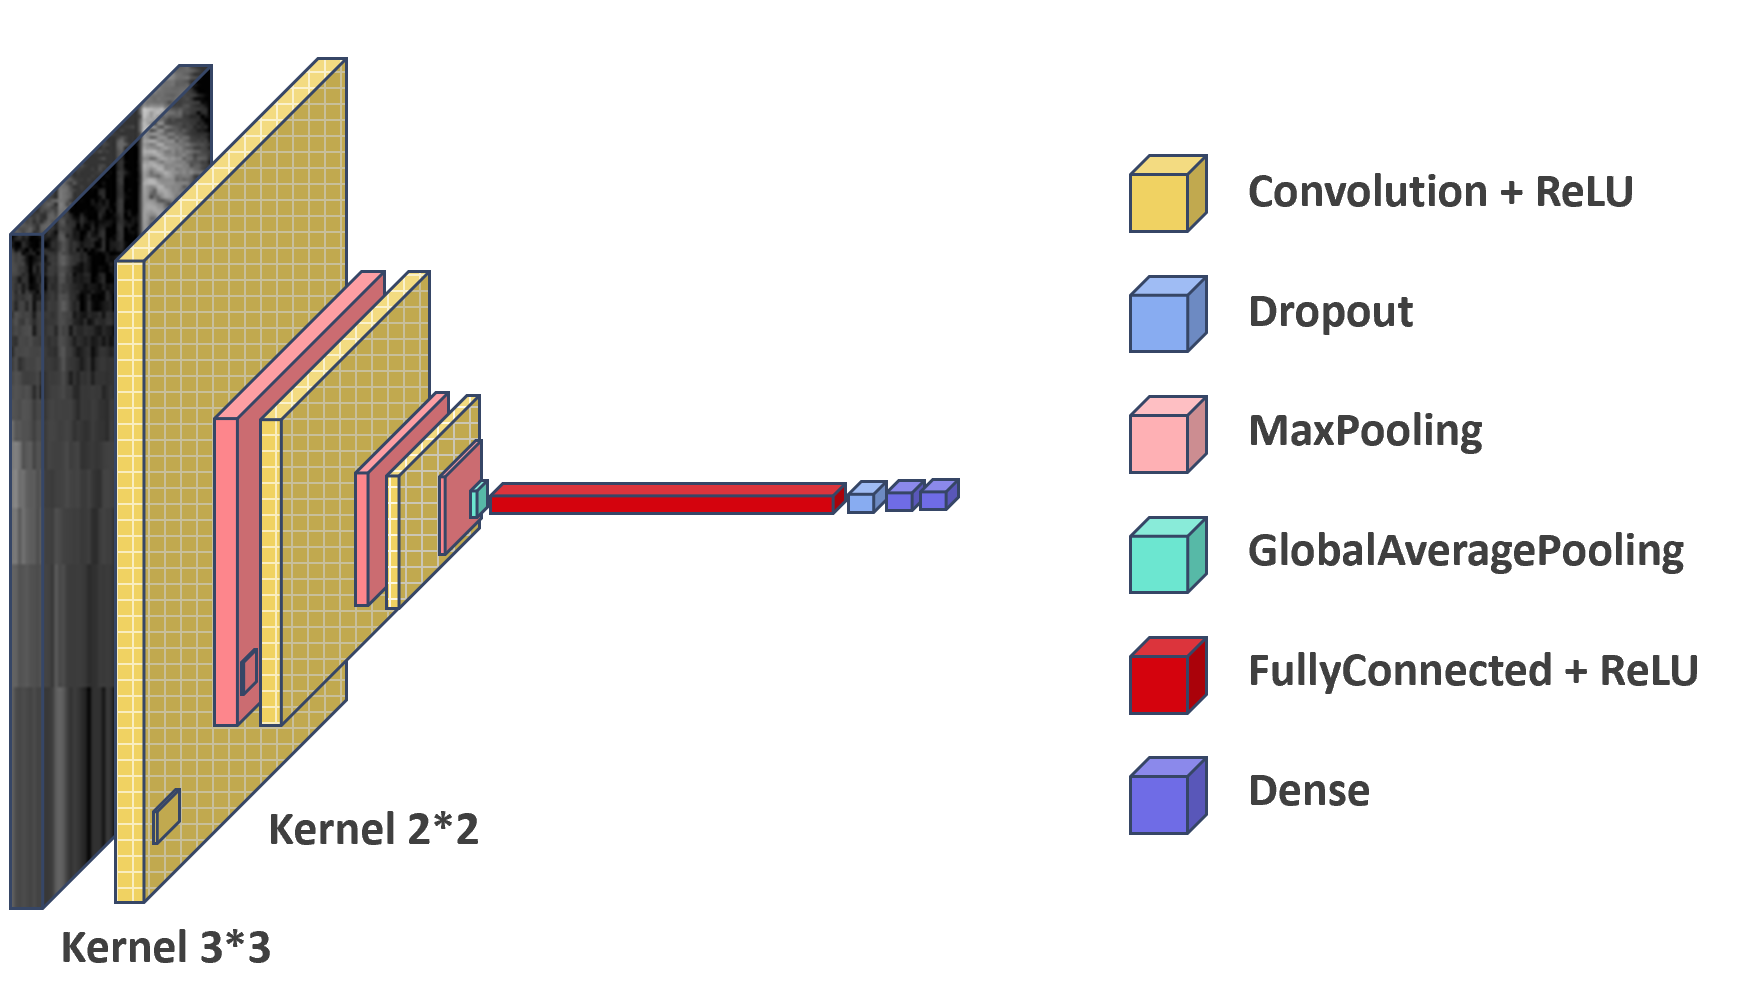
\includegraphics[width=0.8\textwidth]{res/images/cnn/CNNstructure.png}
    \caption{First interface of the SoundRise application}
    \label{fig:soundrise-logo}
\end{figure}

\subsection{Convolutional Layers}
\paragraph{}
Convolutional layers are the core building blocks of CNNs. They apply a set of learnable filters to the input data, producing feature maps that capture various aspects of the input. Each filter is responsible for detecting specific patterns, such as edges or textures, within the data. The convolution operation is defined by parameters such as kernel size, stride, and padding, which influence the spatial dimensions of the output.

\subsection{Pooling Layers}
\paragraph{}
Pooling layers, often interspersed between convolutional layers, serve to reduce the spatial dimensions of the feature maps. This reduction helps to decrease the computational load and control overfitting. The most common type of pooling is max pooling, which selects the maximum value from a defined window, effectively summarizing the presence of a feature. Average pooling is another variant that computes the average value within the window.

\subsection{Fully Connected Layers}
\paragraph{}
After several convolutional and pooling layers, the high-level reasoning in the network is performed by fully connected layers. These layers connect every neuron in one layer to every neuron in the next, similar to a traditional neural network. The final fully connected layer typically outputs a vector of class scores, which are converted into probabilities using a softmax activation function.

\subsection{Activation Functions}
\paragraph{}
Activation functions introduce non-linearity into the network, allowing it to learn complex patterns. The Rectified Linear Unit (ReLU) is the most commonly used activation function in CNNs, defined as \(f(x) = \max(0, x)\). Variants such as Leaky ReLU and Parametric ReLU (PReLU) address some limitations of ReLU by allowing small gradients when the unit is not active.

\paragraph{}
The combination of these layers and functions enables CNNs to automatically learn hierarchical feature representations from input data, making them highly effective for tasks such as image classification, object detection, and more.

\section{Training Core Parameters}
\label{sec:training-parameters}

\paragraph{}
Training a Convolutional Neural Network (CNN) involves several key parameters that significantly influence the model's performance and efficiency. Among these, the number of epochs and batch size are crucial factors that determine the training dynamics and outcomes.

\subsection{Epochs}
\paragraph{}
An epoch refers to one complete pass through the entire training dataset. The number of epochs determines how many times the learning algorithm will work through the dataset. Increasing the number of epochs allows the model to learn more from the data, potentially improving accuracy. However, too many epochs can lead to overfitting, where the model learns the training data too well and performs poorly on unseen data. It is essential to find a balance, often using techniques like early stopping to prevent overfitting by halting training when performance on a validation set starts to degrade.

\subsection{Batch Size}
\paragraph{}
Batch size is the number of training samples processed before the model's internal parameters are updated. A smaller batch size provides a more accurate estimate of the gradient, leading to more stable convergence. However, it can also result in longer training times. Conversely, a larger batch size can speed up training by utilizing parallel processing capabilities of modern hardware, but it may lead to less accurate gradient estimates and potentially poorer generalization. The choice of batch size can also affect the model's ability to escape local minima during training.

\paragraph{}
The interplay between epochs and batch size is critical in determining the training efficiency and effectiveness of a CNN. A well-chosen combination can lead to faster convergence and better model performance, while poor choices can result in longer training times and suboptimal models. Experimentation and cross-validation are often used to find the optimal settings for these parameters.

\section{Key Concepts in CNNs}
\label{sec:key-concepts}

\subsection{Padding}
\paragraph{}
Padding is a technique used in convolutional layers to control the spatial dimensions of the output feature maps. It involves adding extra pixels around the border of the input image or feature map. There are two common types of padding:

\begin{itemize}
    \item \textbf{Valid Padding (No Padding):} In this mode, no padding is added to the input. The convolution operation is applied only to the valid part of the input, which results in a reduction of the spatial dimensions of the output feature map. This is often referred to as "narrow" convolution.
    
    \item \textbf{Same Padding:} In this mode, padding is added to the input so that the output feature map has the same spatial dimensions as the input. This is achieved by adding an appropriate number of zero-pixels around the border of the input. "Same" padding is useful when you want to maintain the spatial dimensions throughout the network, which can be important for certain tasks where spatial resolution is crucial.
\end{itemize}

\subsection{Activation Functions}
\paragraph{}
Activation functions introduce non-linearity into the network, allowing it to learn complex patterns. They are applied element-wise to the output of each layer. Here are some common activation functions used in CNNs:

\begin{itemize}
    \item \textbf{ReLU (Rectified Linear Unit):} Defined as \( f(x) = \max(0, x) \), ReLU is the most commonly used activation function in CNNs. It introduces non-linearity while being computationally efficient. ReLU helps mitigate the vanishing gradient problem, allowing for faster and more effective training of deep networks.
    
    \item \textbf{Leaky ReLU:} A variant of ReLU, Leaky ReLU allows a small, non-zero gradient when the unit is not active (i.e., when \( x < 0 \)). This helps prevent the "dying ReLU" problem, where neurons can become inactive and stop learning.
    
    \item \textbf{Sigmoid and Tanh:} These functions were more commonly used in earlier neural networks. Sigmoid squashes input values to a range between 0 and 1, while Tanh squashes them to a range between -1 and 1. However, they are less commonly used in CNNs due to issues like vanishing gradients.
    
    \item \textbf{Softmax:} Typically used in the output layer of a classification network, softmax converts the raw output scores into probabilities, which sum to 1. This is particularly useful for multi-class classification tasks.
\end{itemize}

\section{Summary}
\label{sec:summary}

\vspace{0.5cm}

\paragraph{}
This chapter has explored the foundational principles of Convolutional Neural Networks (CNNs) and their transformative impact on image classification and beyond. It has highlighted the diverse applications of CNNs across various domains, from medical imaging to natural language processing, showcasing their versatility and effectiveness. The chapter also discussed recent advancements in CNN architectures, including the development of ResNet, MobileNets, and hybrid models, which have further enhanced the capabilities of CNNs. Additionally, the chapter examined the impact of core training parameters such as epochs and batch size, emphasizing their role in optimizing model performance. These insights provide a comprehensive understanding of the current state and future potential of CNNs in addressing complex pattern recognition tasks.